%
% fig-stereographisch.tex
%
% (c) 2024 Prof Dr Andreas Müller
%
\begin{figure}
\centering
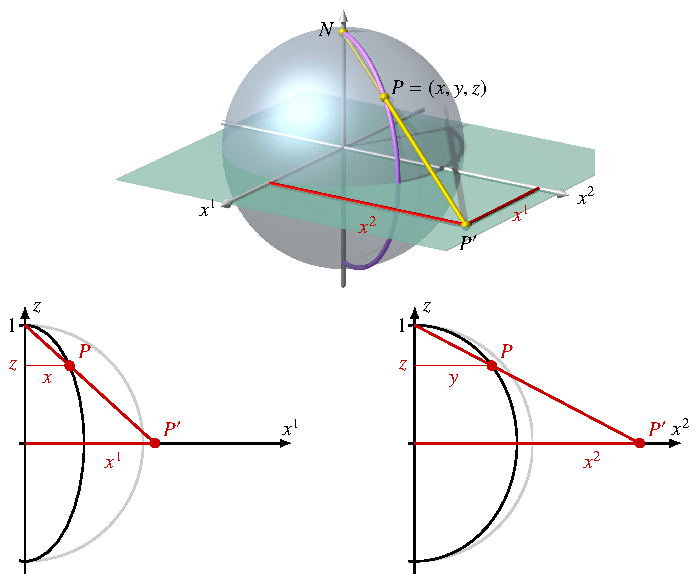
\includegraphics{chapters/020-koordinaten/images/stereographisch.pdf}
\caption{Stereographische Projektion eines Punktes $P$ mit Koordinaten
$(x,y,z)$ auf einer Kugeloberfläche auf die Äquatorebene mit den
Koordinaten $x^1$ und $x^2$.
\label{buch:koordinaten:diffmannig:fig:stereographisch}}
\end{figure}
